%----------------------------------------------------------------------------
\appendix
%----------------------------------------------------------------------------
\chapter*{\fuggelek}\addcontentsline{toc}{chapter}{\fuggelek}
\setcounter{chapter}{\appendixnumber}
%\setcounter{equation}{0} % a fofejezet-szamlalo az angol ABC 6. betuje (F) lesz
\numberwithin{equation}{section}
\numberwithin{figure}{section}
\numberwithin{lstlisting}{section}
%\numberwithin{tabular}{section}

%----------------------------------------------------------------------------
\section{Modellek}
\label{sec:fuggelek}
%----------------------------------------------------------------------------
\subsection{Simple server}

Egy számítógépes szerver modellje, végtelenül leegyszerűsítve. Paramétereink a felhasználói kérések érkezésének rátája, illetve azok kiszolgálásához szükséges idő. Reward függvényeink azt mondják meg, mennyi időt töltünk várakozó állapotban, és hogy milyen gyakorisági rátával tudjuk kiszolgálni az egyes kéréseket.
\begin{center}
	\begin{tabular}{cc}
		\textbf{\textbf{Paraméter}} & \textbf{Default érték} \\
		\hline
		requestRate & 1.5\\
		serviceTime & 0.25\\
	\end{tabular}
	\label{table:filparam}
	\quad
	\begin{tabular}{c}
		\textbf{\textbf{Reward függvény}}\\
		\hline
		Idle\\
		ServedRequests\\
	\end{tabular}
	\label{table:filrewards}
\end{center}
\begin{figure}[!ht]
	\centering
	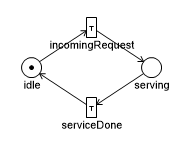
\includegraphics{figures/smpl.png}
	\caption{Egyszerű szerver modellje a PetriDotNet alkalmazásban}
\end{figure}
\clearpage
\subsection{VCL stochastic}

A Virtual Computing Laboratory egy felhő rendszer leegyszerűsített sztochasztikus modellje.
\begin{center}
	\begin{tabular}{lrl}
		\textbf{\textbf{Paraméter}} & \textbf{Default érték} & \textbf{Leírás} \\
		\hline
		incomingRate & 0.015 & Beérkező kérések rátája\\
		dispatchTime & 0.5 & Kérés feldolgozási ideje\\
		warmDispatchTime & 0.15 & További feldolgozási idő meleg gép esetén\\
		jobTime & 60 & Feladatok végrehajtásának átlagos ideje\\
		powerTime & 5 & Gép ki- vagy bekapcsolásának ideje\\
		powerUsage & 0.75 & Gép energiaigénye időegységenként\\
		idlePowerFactor & 0.6 & Várakozó gép energiaigénye\\
	\end{tabular}
	\quad
	\begin{tabular}{ll}
		\textbf{\textbf{Reward függvény}} & \textbf{Leírás}\\
		\hline
		jobsFinished & Befejezett feladatok\\
		powerUsage & Energia felhasználás\\
		noFreeMachines & Szabad gépek hiánya\\
		jobsDispatched & Beérkezett feladatok\\
		machinesWorking & Működő gépek\\
		hotMachinesWorking & Működő meleg gépek\\
		coldStarted & Elindított hideg gépek\\
	\end{tabular}
\end{center}

\begin{figure}
	\centering
	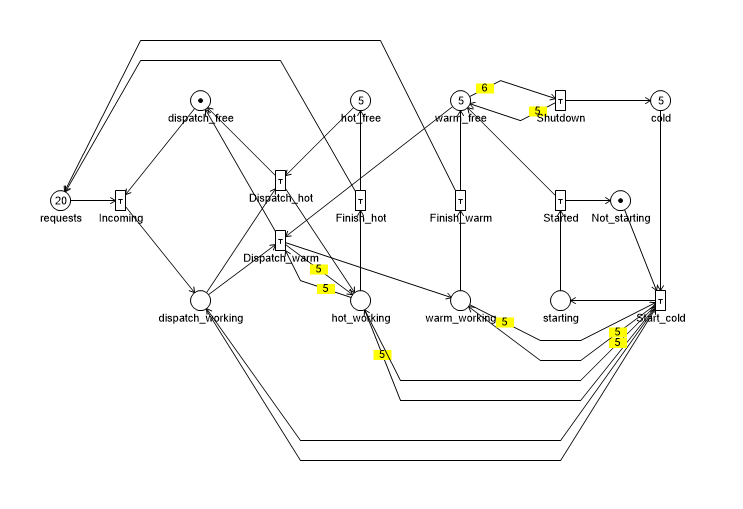
\includegraphics[width=140mm, keepaspectratio]{figures/vcl.png}
	\caption{VCL modell a PetriDotNet alkalmazásban}
\end{figure}

\clearpage
\subsection{Hybrid cloud}

Egy felhő alkalmazás sztochasztikus modellje.
\begin{center}
	\begin{tabular}{lrl}
		\textbf{\textbf{Paraméter}} & \textbf{Default érték} & \textbf{Leírás} \\
		\hline
		incRate & 5& Beérkező kérések rátája\\
		p & 0.75 & A kérés privát felhőhöz érkezésének valószínűsége\\
		lbTime & 0.0002 & Load balancer elindítához szükséges idő\\
		execTime1 & 0.2 & Publikus felhő végrehajtási ideje\\
		execTime2 & 0.1 & Privát felhő végrehajtási ideje\\
		failRate & 0.0002 & Privát szerverek hibarátája\\
		idleFactor & 0.1 & Várakozó gépek relatív igénybevétele\\
		repairTime & 24 & Privát szerverek javítási ideje\\
		publicRent & 0.8 & Óránkénti foglalás publikus felhőn\\
		runPower & 0.3 & Egy működő gép üzemeltetési költsége\\
		idlePower & 0.01 & Egy várakozó gép üzemeltetési költsége\\
		repairCost & 1000 & Gép javításának költsége\\
	\end{tabular}
	\quad
	\begin{tabular}{ll}
		\textbf{\textbf{Reward függvény}} & \textbf{Leírás}\\
		\hline
		Expense & Költség\\
		JobComplete & Teljesített feladatok\\
		JobsProcessing & Folyamatban lévő feladatok\\
		NoFailedServer & Működő szerverek\\
	\end{tabular}
\end{center}

\begin{figure}
	\centering
	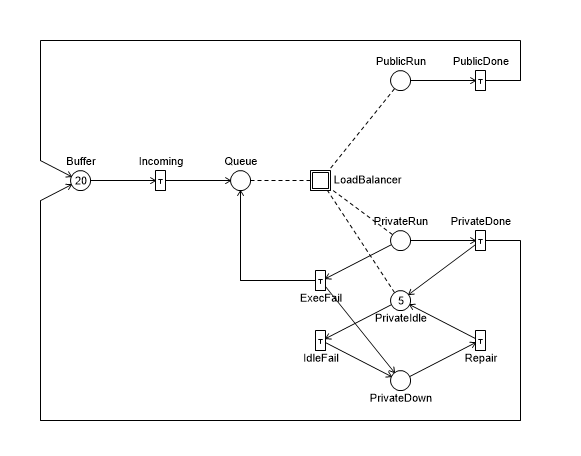
\includegraphics[width=140mm, keepaspectratio]{figures/hybc.png}
	\caption{Hibrid felhő modell a PetriDotNet alkalmazásban}
\end{figure}

\subsection{Philosophers}

A klasszikus ``étkező filozófusok problémája'', stochasztikus rendszerként modellezve.
Adva van valahány filozófus (esetünkben 3, 5, 7 illetve 9), akik egy kerek asztal körül ülnek. Mindegyikük előtt van egy tányér, a tányérok között félúton pedig egy-egy villa. Mindegyik filozófus elmélkedik, egészen addig, míg meg nem éhezik. Akkor azonban csak akkor tud étkezni, ha mindkét oldalán szabad a villa, ha valamelyik nem áll a rendelkezésére, várakoznia kell.

Modelleink esetében a paraméterek jelölik, milyen gyakran éheznek meg az egyes filozófusok, reward függvényeink pedig azt, hogy mennyit tudnak elmélkedni az este folyamán.
\begin{center}
	\begin{tabular}{cc}
		\textbf{\textbf{Paraméter}} & \textbf{Default érték} \\
		\hline
		phil1\_eatingRate & 7.33569408796258\\
		phil2\_eatingRate & 2.15637692896620\\
		phil3\_eatingRate & 9.68078350329879\\
		phil4\_eatingRate & 9.64067749052976\\
		phil5\_eatingRate & 9.47722968486562\\
		phil6\_eatingRate & 4.03202598762859\\
		phil7\_eatingRate & 3.01116461683996\\
		phil8\_eatingRate & 1.24807417152331\\
		phil9\_eatingRate & 6.63293781606486\\
	\end{tabular}
	\label{table:filparam}
	\quad
	\begin{tabular}{c}
		\textbf{\textbf{Reward függvény}}\\
		\hline
		phil1\_thinkingTime\\
		phil2\_thinkingTime\\
		phil3\_thinkingTime\\
		phil4\_thinkingTime\\
		phil5\_thinkingTime\\
		phil6\_thinkingTime\\
		phil7\_thinkingTime\\
		phil8\_thinkingTime\\
		phil9\_thinkingTime\\
	\end{tabular}
	\label{table:filrewards}
\end{center}

\begin{figure}
	\centering
	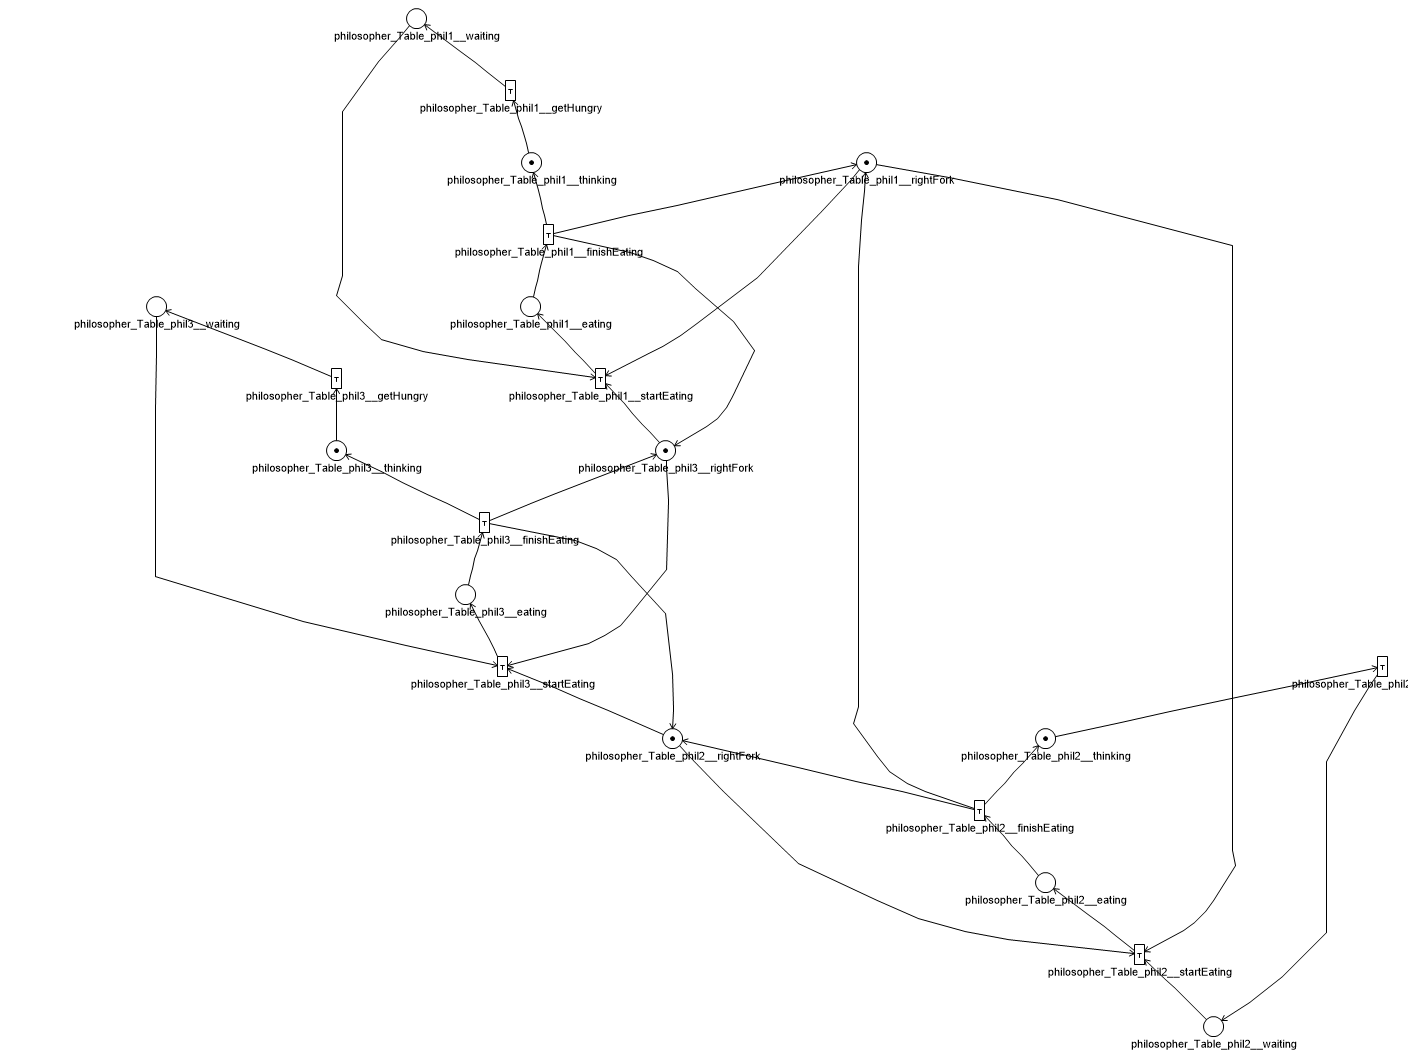
\includegraphics[width=150mm, keepaspectratio]{figures/fil3.png}
	\caption{3 filozófust tartalmazó modell a PetriDotNet alkalmazásban}
\end{figure}